\documentclass{article}
\usepackage{natbib}

\usepackage[margin=1in]{geometry}
\usepackage{lineno,hyperref}
\usepackage{amsmath}
\modulolinenumbers[5]
\usepackage{xcolor}
\usepackage{graphicx}
\usepackage{color}
\usepackage{soul}
\usepackage{longtable}
\usepackage{booktabs}
\usepackage{float}

\renewcommand{\figurename}{Supplemental Figure}

\DeclareMathOperator*{\argmin}{arg\,min}
\def\WIS{\mathrm{WIS}}
\def\rWIS{\mathrm{rWIS}}

%% `Elsevier LaTeX' style
% \bibliographystyle{plain}
\bibliographystyle{model5-names}
%%%%%%%%%%%%%%%%%%%%%%%

\begin{document}

\title{Supplemental Materials for Comparing trained and untrained probabilistic ensemble forecasts of COVID-19 cases and deaths in the United States}

\author{Evan L. Ray
\and
Logan C. Brooks
\and
Jacob Bien
\and
Matthew Biggerstaff
\and
Nikos I. Bosse
\and
Johannes Bracher
\and
Estee Cramer
\and
Sebastian Funk
\and
Aaron Gerding
\and
Michael A. Johansson
\and
Aaron Rumack
\and
Yijin Wang
\and
Martha Zorn
\and
Ryan J. Tibshirani
\and
Nicholas G. Reich}

% \address[umass]{School of Public Health and Health Sciences, University of Massachusetts Amherst}
% \address[cmu]{Machine Learning Department, Carnegie Mellon University}
% \address[usc]{Department of Data Sciences and Operations, University of Southern California}
% \address[kit]{Chair of Statistical Methods and Econometrics, Karlsruhe Institute of Technology}
% \address[hits]{Computational Statistics Group, Heidelberg Institute for Theoretical Studies}
% \address[lshtm]{London School of Hygiene \& Tropical Medicine}
% \address[cdc]{COVID-19 Response, U.S. Centers for Disease Control and Prevention}

\date{}

\maketitle

\linenumbers

\section{Illustration of component forecaster predictive medians}

Supplemental Figures~\ref{fig:component_medians_cases} and \ref{fig:component_medians_deaths} show predictive medians for component forecasts of weekly cases and deaths respectively in selected states with large counts of cases and deaths. We note several important characteristics of the forecasts. For cases, in periods of exponential growth at the start of new waves, it has consistently been the case that two or fewer forecasters accurately predicted that growth. On the other hand, more forecasters have captured periods of growth in deaths.

We also note that for both cases and deaths, there are many outlying forecasts.
These can take the form of forecasts that bear little relation to the observed data, such as forecasts of nearly zero cases near peaks as shown in all facets of Supplemental Figure~\ref{fig:component_medians_cases}, or forecasts that are uniformly too high, such as the outlying forecast of deaths in Florida that is visible in the second panel of Supplemental Figure~\ref{fig:component_medians_deaths}.

Another type of outlying forecast is one that predicts exponential growth that does not materialize, as illustrated at several points in forecasts of cases in Florida and Texas (Supplemental Figure~\ref{fig:component_medians_cases}). We note that these forecasts were unsuccessful, but closely match the trajectories of the few successful forecasts that were made during the Omicron wave in January 2022. This illustrates a potential challenge with automated outlier detection schemes in the context of a process where exponential growth is possible.

\begin{figure}[H]
    \centering
    \includegraphics[width=5.5in]{figures/component_forecast_medians_5_locations_cases.pdf}
    \caption{Component forecasters' predictive medians (blue) for weekly cases (black). For legibility, only the predictive medians originating from every fifth forecast date are shown.}
    \label{fig:component_medians_cases}
\end{figure}

\begin{figure}[H]
    \centering
    \includegraphics[width=5.5in]{figures/component_forecast_medians_5_locations_deaths.pdf}
    \caption{Component forecasters' predictive medians (blue) for weekly deaths (black). For legibility, only the predictive medians originating from every fifth forecast date are shown.}
    \label{fig:component_medians_deaths}
\end{figure}

\newpage

\section{Relative WIS of component forecasters}

Supplemental Figures~\ref{fig:rel_wis_ranks_cases} and \ref{fig:rel_wis_ranks_deaths} show the relative WIS of each component forecaster as a function of the forecast week for the weekly cases and weekly deaths targets respectively. For each week, we calculated a standardized rank for each model based on where that model's relative WIS fell relative to all other models that had submissions that week. In these rankings, 0 indicates the model with the best performance, and 1 indicates the model with the worst performance as measured by relative WIS. We see that nonstationarity of relative performance is very common, with many models alternating between weeks with top-ranking performance and bottom-ranking performance.

Supplemental Figure~\ref{fig:compare_rel_wis_agg_methods} compares two methods for aggregating across forecasters. Recall that as defined in the main text, the relative WIS uses a geometric mean to aggregate WIS ratios across pairs of forecasters. To refresh the notation, we let $\mathcal{I}$ denote a set of combinations of location $l$ and forecast creation date $s$ over which we desire to summarize model performance, and $\mathcal{I}_{m, m'} \subseteq \mathcal{I}$ be the subset of those locations and dates for which both models $m$ and $m'$ provided forecasts. The relative WIS of model $m$ over the set $\mathcal{I}$ is calculated as
\begin{align*}
\rWIS^{m,geom}_{\mathcal{I}} &= \frac{\theta^m}{\theta^{\text{baseline}}} \text{, where } \\
\theta^m &= \left(\prod_{m'=1}^M \frac{(4 \cdot \vert \mathcal{I}_{m, m'} \vert)^{-1} \sum_{(l, s) \in \mathcal{I}_{m, m'}} \sum_{t=s+1}^{s+4} \WIS(q^m_{l,s,t,1:K},y_{l,t}) }{ (4 \cdot \vert \mathcal{I}_{m, m'} \vert)^{-1} \sum_{(l, s) \in \mathcal{I}_{m, m'}} \sum_{t=s+1}^{s+4} \WIS(q^{m'}_{l,s,t,1:K},y_{l,t})} \right)^{\frac{1}{M}}.
\end{align*}
The figure compares to the alternate strategy of using an arithmetic mean to aggregate across model pairs:
\begin{align*}
\rWIS^{m,arith}_{\mathcal{I}} &= \frac{\theta^m}{\theta^{\text{baseline}}} \text{, where } \\
\theta^m &= \frac{1}{M}\sum_{m'=1}^M \frac{(4 \cdot \vert \mathcal{I}_{m, m'} \vert)^{-1} \sum_{(l, s) \in \mathcal{I}_{m, m'}} \sum_{t=s+1}^{s+4} \WIS(q^m_{l,s,t,1:K},y_{l,t}) }{ (4 \cdot \vert \mathcal{I}_{m, m'} \vert)^{-1} \sum_{(l, s) \in \mathcal{I}_{m, m'}} \sum_{t=s+1}^{s+4} \WIS(q^{m'}_{l,s,t,1:K},y_{l,t})}.
\end{align*}
There is no substantive difference between the relative WIS values obtained using these aggregation strategies.


\begin{figure}[H]
    \centering
    \includegraphics[width=5.5in]{figures/rel_wis_ranks_cases.pdf}
    \caption{Weekly component ranks according to relative WIS for forecasts of cases in the U.S. A rank of 0 indicates that the model has the best performance in a given week, and a rank of 1 indicates that it has the worst performance. There is a facet for each component forecaster, and the colored line shows the standardized rank of that forecaster.}
    \label{fig:rel_wis_ranks_cases}
\end{figure}

\begin{figure}[H]
    \centering
    \includegraphics[width=5.5in]{figures/rel_wis_ranks_deaths.pdf}
    \caption{Weekly component ranks according to relative WIS for forecasts of deaths in the U.S. A rank of 0 indicates that the model has the best performance in a given week, and a rank of 1 indicates that it has the worst performance. There is a facet for each component forecaster, and the colored line shows the standardized rank of that forecaster.}
    \label{fig:rel_wis_ranks_deaths}
\end{figure}

\begin{figure}[H]
    \centering
    \includegraphics[width=5.5in]{figures/compare_wis_agg_methods.pdf}
    \caption{Comparison of aggregation methods used to summarize across models when calculating the relative WIS. Each point corresponds to one combination of component forecaster and forecast date, and shows the relative WIS based on a trailing window of 12 weeks using the arithmetic mean to summarize across models (horizontal axis) or the geometric mean to summarize across models (vertical axis). The figure shows these results for all component model forecasts of incident cases at the state level in the United States made on dates between July 27, 2020 and March 14, 2022 using the truth data available as of the forecast date; the relative WIS scores shown are those that would have been used as input to the relative WIS weighted ensemble methods for real-time forecasts.}
    \label{fig:compare_rel_wis_agg_methods}
\end{figure}

\newpage

\section{Comparison of logarithmic score and weighted interval score}

In the Forecast Hubs, all forecasts are represented by a set of predictive quantiles at specified probability levels. This has motivated our decision to use the weighted interval score (WIS) for forecast evaluation, as the WIS is a proper score for quantile forecasts. In this section, we discuss challenges with using the logarithmic score when only predictive quantiles are available, and give a qualitative illustration of the difference between the logarithmic score and the WIS. We give a general discussion in Section~\ref{subsec:log_score_wis_example}, and defer some technical details to Section~\ref{subsec:log_score_wis_extrapolation_methods}.

\subsection{Illustrative example comparing the logarithmic score and WIS}
\label{subsec:log_score_wis_example}

Suppose that we have a forecast submission consisting of quantiles of a predictive distribution at the 23 probability levels used in the Forecast Hub, and our goal is to calculate a score that measures the accuracy of this forecast for the observed value $y_{obs}$. One common choice of score for probabilistic forecasts is the logarithmic score; here we consider the negative logarithmic score so that its orientation matches that of the WIS. If a predictive density $f_Y(y)$ is available, the negative logarithmic score is defined as

$$NLS(f_Y, y_{obs}) = -\log[f_Y(y_{obs})]$$

In a setting where we do not have the predictive density $f_Y$, but only predictive quantiles, the logarithmic score cannot be calculated. One possible route forward is to attempt to reconstruct the predictive density from the provided predictive quantiles. We illustrate here that within the limits of the predictive quantiles, it is possible to obtain a reasonable approximation of the predictive density. Here, we do so by fitting a monotonic spline to the provided quantiles to approximate the cumulative distribution function, and then differentiating to approximate the probability density function. However, extrapolating beyond the predictive quantiles is more of a challenge, and requires some assumption to be made about the behavior of the tails of the predictive distribution. This assumption can have a large impact on the log score when observations fall in the tails.

Supplemental Figure~\ref{fig:log_score_and_wis} illustrates this using an example of a hypothetical forecast submission consisting of quantiles of the predictive distribution $Y \sim \text{log normal}(4, 0.5)$. We compare this predictive distribution with two approximations of it that are derived from the quantiles: one assuming a normal distribution for the tails, and the second assuming a Cauchy distribution for the tails. Although there are apparently only minor differences in the CDFs and PDFs of these distributions, the log scores diverge substantially in the tails. By construction, all three distributions have the same quantiles at the 23 points that were included in the submission, and so the WIS is identical for all three distributions. To summarize, when only a set of predictive quantiles are provided, there is not enough information to characterize the behavior of the forecast distribution in the tails, and so a log score cannot be calculated. On the other hand, the WIS is defined only in terms of the specified predictive quantiles, and so it does not suffer from this problem.

\begin{figure}
    \centering
    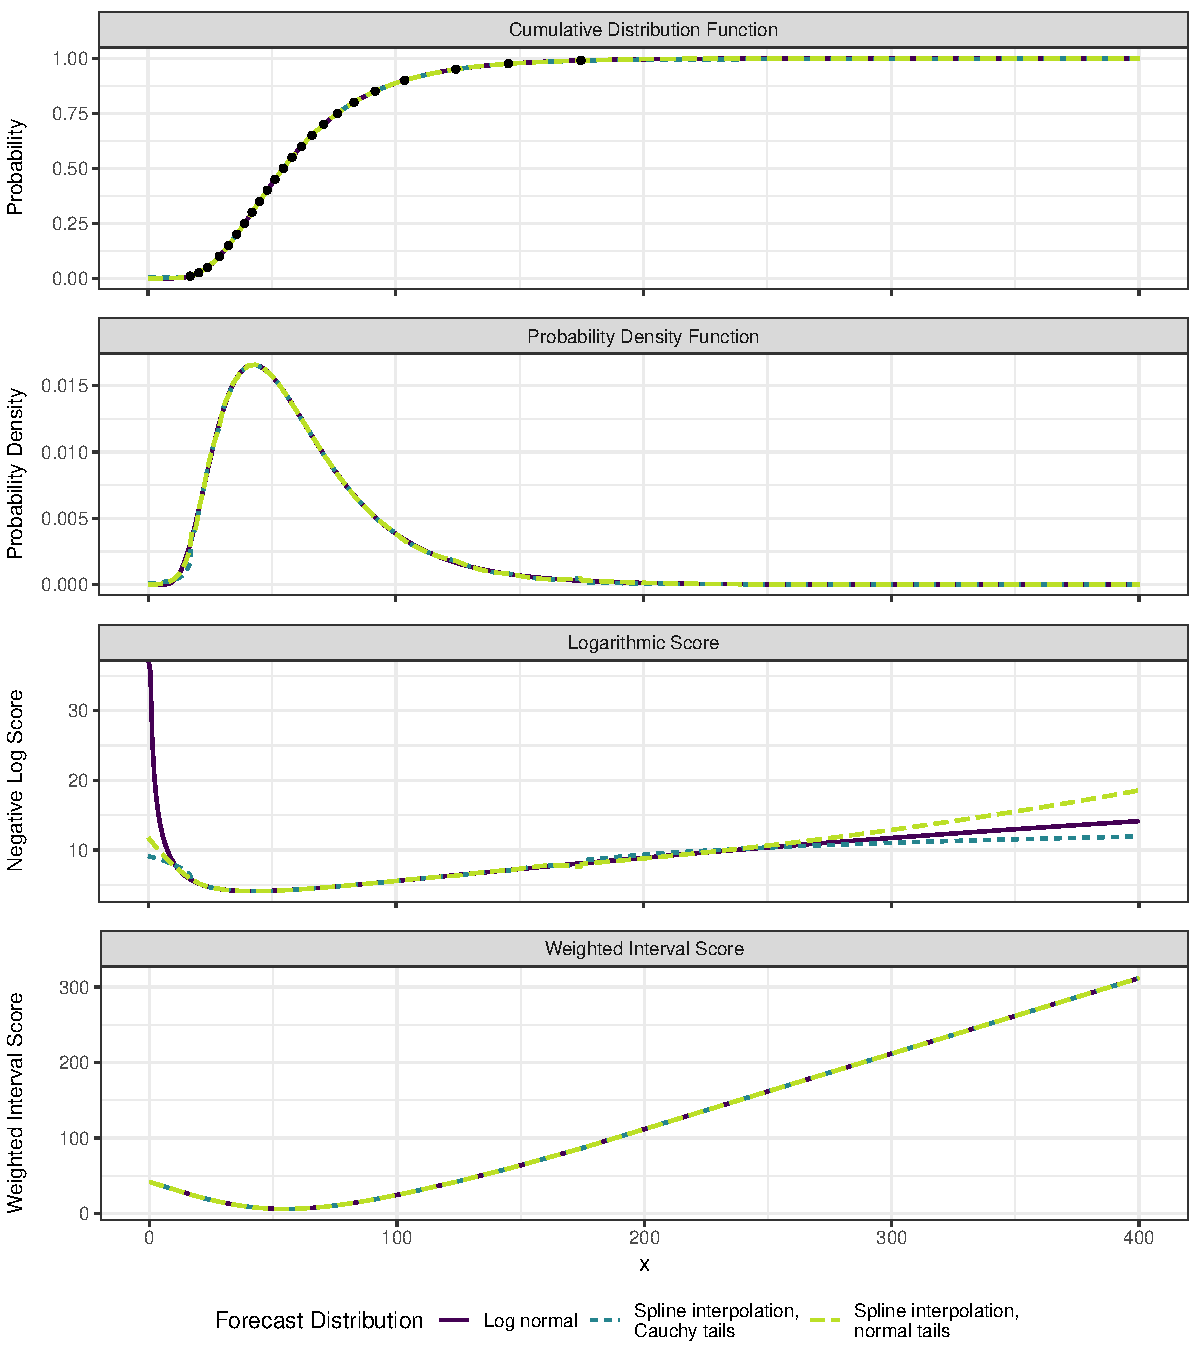
\includegraphics[width=\textwidth]{figures/log_score_and_wis.pdf}
    \caption{CDFs, PDFs, log scores, and WIS for a $\text{log normal}(4, 0.5)$ forecast and two approximations to it that match 23 specified quantiles but have different behavior in the tails. The predictive quantiles are shown with black points in the top panel.}
    \label{fig:log_score_and_wis}
\end{figure}

Qualitatively, the figure shows that both the negative log score and the WIS are minimized when the observed value falls near the center of the predictive distribution, and are larger when the observation falls in the tails. More formally, the negative log score is optimized when the observed value falls at a predictive mode, while the weighted interval score is optimized when the observed value falls at the predictive median. See \cite{bracherEvaluatingEpidemicForecasts2021} for additional discussion of these scores and the continuous ranked probability score.

\subsection{Methods for approximating a predictive density based on predictive quantiles}
\label{subsec:log_score_wis_extrapolation_methods}

Here we describe the methods used in the previous section for obtaining an approximate predictive density $\hat{f}_Y$ based on a set of predictive quantiles $q_1, \ldots, q_K$ at probability levels $\tau_1, \ldots, \tau_K$. The method works in two phases: (1) we estimate the density on the interior of the predictive quantiles as the derivative of a monotonic spline that estimates the CDF; and (2) we approximate the tails with a distribution in a specified location-scale family.

For the interior points, we fit a monotonic spline that interpolates the set of ``observations'' $\{(q_1, \tau_1), \ldots, (q_K, \tau_K)\}$. This spline is an estimate of the predictive CDF, and its derivative estimates the predictive PDF. Because the spline passes through the points $(q_1, \tau_1)$ and $(q_K, \tau_K)$, the integral of its derivative over the interval $[q_1, q_K]$ is equal to $\tau_K - \tau_1$.

We estimate the density for the left and right tails separately, assuming that they come from a specified location-scale family. Setting notation, suppose that $Y = a + b \cdot Z$ where the random variable $Z$ has a specified distribution. Recall that at the probability level $\tau$, a quantile of $Y$ can be calculated in terms of the corresponding quantile of $Z$ via $q_Y(\tau) = a + b \cdot q_Z(\tau)$. Using the quantiles at two probability levels $\tau_i$ and $\tau_j$, we can calculate the value of $b$ using

\begin{align*}
\frac{q_Y(\tau_i) - q_Y(\tau_j)}{q_Z(\tau_i) - q_Z(\tau_j)} &= \frac{a + b \cdot q_Z(\tau_i) - (a + b \cdot q_Z(\tau_j))} {q_Z(\tau_i) - q_Z(\tau_j)} \\
&= b \cdot \frac{q_Z(\tau_i) - q_Z(\tau_j)}{q_Z(\tau_i) - q_Z(\tau_j)} \\
&= b
\end{align*}

Similarly, we can calculate the value of $a$ as

$$q_Y(\tau_i) - b \cdot q_Z(\tau_i) = a + b \cdot q_Z(\tau_i) - b \cdot q_Z(\tau_i) = a$$

In the above expressions, we use the two smallest quantiles when estimating the lower tail and the two largest quantiles when estimating the upper tail. With these choices, by construction the lower tail integrates to $\tau_1$ on the interval $(-\infty, q_1]$ and the upper tail integrates to $1 - \tau_K$ on the interval $[q_K, \infty)$.

\newpage

\section{Quantile ensembles as horizontal combinations of predictive CDFs}

Supplemental Figure \ref{fig:ensemble_cdf_combination} illustrates the ensemble methods considered in this manuscript as horizontal combinations of the cumulative distribution functions of predictive distributions from component forecasters, computing a weighted or unweighted mean or median at each quantile probability level along the vertical axis.

\begin{figure}[H]
    \centering
    \includegraphics[width=\textwidth]{figures/ensemble_cdf_combination.pdf}
    \caption{Illustration of four ensemble methods for forecasting incident deaths in Ohio at a forecast horizon of 1 week from February 15, 2021. Each line corresponds to the forecast distribution from one component model or ensemble, and is obtained by interpolating between the 23 predictive quantiles; the resulting curves approximate the predictive CDFs associated with these forecasts. The curves are cut off for two component forecasters with extremely wide predictive distributions. At each quantile level along the vertical axis, the ensemble forecasts are obtained as a combination of the component model forecasts at that quantile level.}
    \label{fig:ensemble_cdf_combination}
\end{figure}

\newpage

\section{Expanded results from primary analysis}

This section includes figures giving additional views of the primary results from Figures 3, 4, 5, and 7 in the article.

\subsection{Full distributions of Weighted Interval Score differences}

For legibility, Figures 3 and 7 in the main text displayed the central tendency (central quantiles and means) of differences in weighted interval scores between the different methods, but suppressed outliers corresponding to individual combinations of forecast dates and horizons with large differences between the equal weighted median ensemble and another ensemble method. Supplemental Figures \ref{fig:wis_boxplots_by_phase_all_points_us} and \ref{fig:wis_boxplots_by_phase_all_points_eu} display full box plots including outliers that were suppressed in the main text.

\begin{figure}[H]
\includegraphics[width=\textwidth]{figures/wis_boxplots_by_phase_US_all_points.pdf}
\caption{Performance measures for ensemble forecasts of weekly cases and deaths in the U.S. The vertical axis is the difference in mean WIS for the given ensemble method and the equally weighted median ensemble.
Boxplots summarize the distribution of these differences in means, averaging across all locations for each combination of forecast date and horizon.
A cross is displayed at the difference in overall mean scores for the specified combination method and the equally weighted median averaging across all locations, forecast dates, and horizons.
A negative value indicates that the given method outperformed the equally weighted median.
}
\label{fig:wis_boxplots_by_phase_all_points_us}
\end{figure}

\begin{figure}[H]
\includegraphics[width=\textwidth]{figures/wis_boxplots_by_phase_EU_all_points.pdf}
\caption{Performance measures for ensemble forecasts of weekly cases and deaths in Europe. The vertical axis is the difference in mean WIS for the given ensemble method and the equally weighted median ensemble.
Boxplots summarize the distribution of these differences in means, averaging across all locations for each combination of forecast date and horizon.
A cross is displayed at the difference in overall mean scores for the specified combination method and the equally weighted median averaging across all locations, forecast dates, and horizons.
A negative value indicates that the given method outperformed the equally weighted median.
}
\label{fig:wis_boxplots_by_phase_all_points_eu}
\end{figure}

\newpage

\subsection{Scores by forecast creation date}

Supplemental Figures \ref{fig:rel_WIS_over_time_us} and \ref{fig:rel_WIS_over_time_euro} show relative WIS for the ensemble methods over time for forecasts in the US and in Europe respectively.
The included ensemble methods are 1) an equally weighted mean ensemble, 2) an equally weighted median ensemble, 3) a weighted mean ensemble, and 4) a weighted median ensemble.
Both of the weighted ensembles combine the ten component forecasters with best individual performance as measured by the relative WIS, and are trained on a sliding 12-week window.
The component forecasters included in the trained ensembles are updated each week based on performance during the training window.
  
\begin{figure}
  \includegraphics[width=6in]{figures/rel_wis_by_week_US.pdf}
  \caption{Weekly reported cases and deaths at the national level in the United States and mean weighted interval scores (WIS) relative to the baseline for state-level forecasts over time for four ensembles.
  Mean WIS is calculated separately for each combination of forecast horizon and forecast creation date, averaging across all states and territories, and then normalized relative to the mean WIS for the baseline model.
  Lower scores indicate better forecast performance.
  A vertical dashed line is shown at the start of the prospective evaluation phase.
  }
  \label{fig:rel_WIS_over_time_us}
\end{figure}

\begin{figure}
  \includegraphics[width=6in]{figures/rel_wis_by_week_EU.pdf}
  \caption{Weekly reported cases and deaths aggregated across all European countries included in the European Forecast Hub and mean weighted interval scores (WIS) relative to the baseline for state-level forecasts over time for four ensembles.
  Mean WIS is calculated separately for each combination of forecast horizon and forecast creation date, averaging across all states and territories, and then normalized relative to the mean WIS for the baseline model.
  Lower scores indicate better forecast performance.
  A vertical dashed line is shown at the start of the prospective evaluation phase.
}
  \label{fig:rel_WIS_over_time_euro}
\end{figure}

\newpage

\subsection{95\% prediction interval widths}

Supplemental Figures~\ref{fig:95_pi_width_cases} and \ref{fig:95_pi_width_deaths} illustrate that the widths of 95\% prediction intervals for the ensemble forecasters generally fall in the middle of the widths of the intervals from the component forecasters. This is true because the ensemble forecasts are a (weighted) mean or median of predictive quantiles of the component forecasters. In particular, the equal weighted median forecast typically has a 95\% interval width that ranks very close to the middle of the other forecasters' interval widths.

We note that interval coverage rates are not in themselves a measure of forecast skill, and it is important to also consider whether the interval contains the forecasted quantity at the nominal coverage rate (i.e., whether the forecasts are well-calibrated). The figures in the main text include displays of calibration as well as proper scores that measure both calibration and sharpness together.

\begin{figure}
  \includegraphics[width=6in]{figures/95_PI_width_ranks_cases.pdf}
  \caption{Standardized ranks of 95\% prediction intervals for weekly cases from component forecasters, the equally weighted median ensemble, and the relative WIS weighted median ensemble. For each combination of location, forecast date, and forecast horizon, we rank the widths of 95\% prediction intervals from all forecasters that submitted the relevant forecast on a scale from 0 to 1, where the forecaster with the narrowest interval has rank 0 and the forecaster with the widest interval has rank 1. Density plots summarize the distribution of these ranks for each forecaster; forecasters are sorted by their median rank.}
  \label{fig:95_pi_width_cases}
\end{figure}


\begin{figure}
  \includegraphics[width=6in]{figures/95_PI_width_ranks_deaths.pdf}
  \caption{Standardized ranks of 95\% prediction intervals for weekly deaths from component forecasters, the equally weighted median ensemble, and the relative WIS weighted median ensemble. For each combination of location, forecast date, and forecast horizon, we rank the widths of 95\% prediction intervals from all forecasters that submitted the relevant forecast on a scale from 0 to 1, where the forecaster with the narrowest interval has rank 0 and the forecaster with the widest interval has rank 1. Density plots summarize the distribution of these ranks for each forecaster; forecasters are sorted by their median rank.}
  \label{fig:95_pi_width_deaths}
\end{figure}

\newpage

\subsection{Impact of reporting anomalies}

We conducted a supplemental analysis in which we removed forecasts that were affected by reporting anomalies before calculating summaries of forecast performance. We catalogued two types of reporting anomalies, as illustrated in Supplemental Figure~\ref{fig:anomalies_example}:
\begin{enumerate}
    \item \textbf{Outliers} were identified manually by examining plots of the data. Negative weekly counts and other observations that did not appear to match local trends were recorded as outliers.
    \item \textbf{Revisions} were identified automatically. The value for a particular week was identified as a large revision if the difference between the original reported value and the final reported value was at least 20, and that difference was at least 40\% of the initial reported value or the final reported value.
\end{enumerate}

\begin{figure}
  \includegraphics[width=\textwidth]{figures/anomalies_example-inc-deaths-US.pdf}
  \caption{An illustration of data anomalies identified for weekly deaths in the state of Texas. Identified outliers include suppressed reporting during holidays and a winter storm in February 2021, as well as a period of reduced reporting followed by catch-up reporting in October 2021.}
  \label{fig:anomalies_example}
\end{figure}

For the purpose of this analysis, forecasts with a target end date coinciding with an observation that was identified as an outlier were excluded. This is because we would prefer forecasting methods to focus on capturing the epidemiological process rather than aspects of the reporting process that lead to outliers.

Forecasts with a forecast date on the date of a value that was later revised, or within the following 3 weeks unless the revision had already been made by the time of the forecast, were excluded. These forecasts were excluded because the input data used for the forecast were not a reliable indicator of the state of the epidemic at the time of the forecast. One might reasonably expect forecasters to account for the possibility of such data revisions, but this analysis represents a conservative examination of whether these revisions affected the main results in the article.

Together, these criteria led to removal of 531 combinations of location, forecast date, and forecast horizon out of 19,256 such combinations throughout the model development and prospective evaluation phases in the U.S.

Supplemental Figures~\ref{fig:wis_calibration_us_non_anomalous} and \ref{fig:wis_calibration_us_non_anomalous_all_points} mirror Figure 3 in the primary text and Supplemental Figure~\ref{fig:wis_boxplots_by_phase_all_points_us}, summarizing forecast skill after removing scores affected by reporting anomalies. Although the forecasts affected by reporting anomalies generally had higher WIS values than other forecasts, they did not have unusually large \textit{differences} in WIS between forecasting methods. The results about the relative performance of ensemble methods hold stable whether or not the forecasts affected by data anomalies are removed.

\newpage

\begin{figure}[H]
  \includegraphics[width=\textwidth]{figures/wis_boxplots_and_calibration_by_phase_US_central_only_non_anomalous.pdf}
  \caption{Summaries of forecast performance after removing forecasts affected by reporting anomalies. Panel (a) shows the 25th percentile, median, and 75th percentile of differences in mean WIS between specified ensemble methods and the equally weighted median ensemble, where the means average across locations for each combination of forecast date and forecast horizon. Crosses show the difference in overall mean WIS averaging across all locations, forecast dates, and forecast horizons. Panel (b) shows the calibration of predictive quantiles, with the difference between the empirical coverage rate and the nominal coverage rate on the vertical axis. A well calibrated model will have a difference between the empirical coverage rate and the nominal quantile level that is approximately zero. A method that generates conservative two-sided intervals would have a difference that is negative for nominal quantile levels less than 0.5 and positive for nominal quantile levels greater than 0.5.}
  \label{fig:wis_calibration_us_non_anomalous}
\end{figure}

\begin{figure}[H]
  \includegraphics[width=\textwidth]{figures/wis_boxplots_by_phase_US_all_points_non_anomalous.pdf}
  \caption{Summaries of forecast performance after removing forecasts affected by reporting anomalies. Boxplots summarize the distribution of differences in mean WIS between specified ensemble methods and the equally weighted median ensemble, where the means average across locations for each combination of forecast date and forecast horizon. Crosses show the overall difference in mean WIS averaging across all locations, forecast dates, and forecast horizons.}
  \label{fig:wis_calibration_us_non_anomalous_all_points}
\end{figure}

\newpage

\section{Model variations considered during development phase}

Here we present some results for model variations considered during the model development phase. All figures here represent only scores for forecast dates before May 3, 2021.

\subsection{Additional combination methods and training window sizes}

The manuscript gives results for equally weighted mean and median ensembles, and relative WIS weighted mean and median ensembles, using a fixed training set window size of the 12 weeks prior to the forecast date. Here we show results on the development set for forecasts using a range of training set window sizes including 4 weeks, 8 weeks, 12 weeks, and all available forecast history. We also consider two additional combination methods along with those presented in the main text.

The first of these new combination methods is a weighted mean. As a reminder,  $q^m_{l,s,t,k}$ denotes the predictive quantile at probability level $k$ from component model $m$ at location $l$, forecast date $s$, and target end date $t$. With this notation, the weighted mean ensemble forecast quantiles are calculated as
$$q^\text{ens}_{l,s,t,k} = \sum_{m = 1}^M w^m_{s} q^{m}_{l,s,t,k}.$$
The model weights $w^m_s$ are constrained to be non-negative and sum to one; in case of missing forecasts, the weights for any missing models are set to zero and the remaining weights are rescaled to sum to 1.
As indicated by the subscript $s$, the weights $w^m_s$ are updated each week by optimizing the ensemble WIS over the training window of the specified number of weeks before the forecast date $s$.

The second of the new combination methods is a weighted median ensemble that uses the weights estimated for the weighted mean ensemble. This offers comparable flexibility to the weighted mean ensemble, but has the disadvantage that the weights are not obtained by optimizing the forecast skill of the method that is actually used for forecast combination. Direct estimation of the weights for a weighted median by optimizing ensemble WIS is challenging because the objective function is not differentiable in the weights; the optimization problem is a mixed integer linear program, which is computationally demanding. In other experiments, we also considered a method for computing an approximate weighted median by the smoothing weighted distribution of predictive quantiles from component forecasters. However, this method's performance was not substantively different from the other methods considered here and we omit those results for brevity.

Supplemental Figures~\ref{fig:wis_combination_methods_central_only} and \ref{fig:wis_combination_methods_all_points} display the results of this expanded comparison including all combinations of the training set window size, the six combination methods, and three variations on the number of top-performing component forecasters included in the ensemble. Across all combinations of training set window size, number of component forecasters included, and target variable (cases or deaths), the relative WIS weighted median ensemble had the most stable performance. For deaths, it had the best mean WIS for all training set window sizes, though it had similar performance to the equally weighted median of the top 5 models. For cases, it was more often matched by other methods, though the performance of the other methods was more inconsistent across different settings for other tuning parameters. Across most settings, using a relative WIS weighted mean or median offered an improvement in mean WIS over taking an equally weighted mean or median of top performing models.

There is perhaps a slight indication that an intermediate training set size of 8 to 12 weeks is better than training on 4 weeks or the full available history, but this signal is not strong. Some of the combination methods were better when fewer top models were included, but the relative WIS weighted median method was not sensitive to this setting.

We selected the relative WIS weighted mean and median ensembles for the prospective evaluation because they were consistently better than both more flexibly weighted methods and equally weighted combinations of top-performing components when forecasting cases, and were comparable to the best of the other approaches when forecasting deaths. We selected an intermediate training set window size of 12 weeks because both the relative WIS weighted mean and median methods did well with that training set size. We selected including the top ten component forecasters as an intermediate setting for that tuning parameter, though we did not see a strong reason to prefer it to the other possibilities we considered.

\newpage

\begin{figure}[H]
  \includegraphics[width=\textwidth]{figures/wis_boxplots_all_combos_central_only.pdf}
  \caption{The 25th percentile, median, and 75th percentile of differences in mean WIS between specified ensemble methods and the equally weighted median of all component forcasters, where the means average across locations for each combination of forecast date and forecast horizon. Crosses show the overall difference in mean WIS averaging across all locations, forecast dates, and forecast horizons.
  A negative value indicates that the method corresponding to a particular combination of training set size, number of component forecasters included, and combination method outperformed the ensemble calculated as an equally weighted median of all component forecasts.}
  \label{fig:wis_combination_methods_central_only}
\end{figure}


\begin{figure}[H]
  \includegraphics[width=\textwidth]{figures/wis_boxplots_all_combos_all_points.pdf}
  \caption{Boxplots summarizing the full distribution of differences in mean WIS between specified ensemble methods and the equally weighted median of all component forcasters, where the means average across locations for each combination of forecast date and forecast horizon. Crosses show the overall difference in mean WIS averaging across all locations, forecast dates, and forecast horizons.
  A negative value indicates that the method corresponding to a particular combination of training set size, number of component forecasters included, and combination method outperformed the ensemble calculated as an equally weighted median of all component forecasts.}
  \label{fig:wis_combination_methods_all_points}
\end{figure}


\subsection{Separate weights at different forecast horizons}

We considered a variation on the relative WIS weighted median ensemble that estimated separate weights for each of the one through four week ahead forecast horizons. In this approach, the relative WIS of component forecasters was calculated separately at each forecast horizon, and the estimation of the weighting parameter $\theta$ was performed separately to optimize the forecast skill of the ensemble at each horizon.

Supplemental Figure~\ref{fig:wis_grouping_by_horizon} shows the results of this per-horizon weighting scheme for the relative WIS weighted median ensemble combining the top 10 component forecasters. We found that using separate model weights at each forecast horizon led to small improvements in mean WIS at short-term forecast horizons of one to two weeks ahead, but slightly worse mean WIS at longer forecast horizons of three to four weeks ahead. 

We see two possible contributing factors to these results. First, forecasts at long horizons have scores that are larger in magnitude than forecasts at short horizons, and so tend to dominate the overall score when averaging across horizons. This may result in weights that favor performance at longer term horizons when weights are shared across horizons, thereby harming performance of forecasts at short horizons. Second, sharing weights across horizons may be particularly helpful for longer term forecasts because of the gain in the training set sample size that comes with weight sharing. For example, with a training set size of four weeks and weights estimated separately by horizon, only one week's worth of forecasts are actually included in the training set for weight estimation at a horizon of four weeks, because the target data for four-week ahead forecasts made within the past three weeks have not yet been observed at the time of weight estimation. Sharing weights across horizons means that more information about model performance is available for weight estimation at these longer horizons. In support of this explanation, note that the magnitude of relative losses in forecast skill from estimating per-horizon weights at longer forecast horizons decreases as the training set size increases.

These results suggest the possibility of a blended strategy, where per-horizon estimation is used to obtain the weights for short horizons but the weights for longer horizons are estimated by sharing information across all horizons. In light of the small magnitude of the gains from using a per-horizon weighting at short horizons, we decided to pursue a unified approach of using shared weights across all horizons to reduce methodological and narrative complexity.

\begin{figure}
  \includegraphics[width=\textwidth]{figures/wis_boxplots_horizon_grouping.pdf}
  \caption{Boxplots summarizing forecast skill for forecasts of weekly cases, varying whether model weights are shared across all forecast horizons or are estimated separately for each forecast horizon.
  The vertical axis is the difference in mean skill for the given ensemble specification when component weights are shared across all horizons and the same specification with separate component weights for each forecast horizon.
  The boxplots summarize the distribution of these differences for each combination of forecast date and horizon, averaging across all locations.
  A cross is displayed at the difference in overall mean scores.
  A negative value indicates that the method with separate component weights for each forecast horizon outperformed the corresponding specification with weights shared across forecast horizons.
  For this analysis, only results for relative WIS weighted ensembles combining the ten best individual component forecasters are presented.}
  \label{fig:wis_grouping_by_horizon}
\end{figure}

\newpage

\subsection{Separate weights at different quantile levels}

We considered strategies for estimation of separate model weights at each quantile level rather than sharing model weights across all quantile levels.
We considered this possibility for both the relative WIS weighted median ensemble and the convex mean ensemble that directly optimizes the component weights rather than setting them to be a sigmoid function of the relative WIS.
In both variations, weights were estimated by optimizing the contribution to the WIS from each quantile level separately, i.e., the pinball loss.
Similarly, for the relative WIS weighted median, the relative WIS for component models that is used as an input for calculating model weights was obtained separately based on the contribution to WIS at each quantile level.

Supplemental Figures~\ref{fig:wis_quantile_grouping_rel_wis} and \ref{fig:wis_quantile_grouping_convex} summarize the WIS of these methods on the model development set, comparing these approaches to the corresponding methods with a single weight per model that is shared across all quantile levels. Supplemental Figure~\ref{fig:coverage_quantile_grouping} displays the probabilistic calibration of these model variations in terms of one-sided coverage rates for predictive quantiles. In this experiment, all methods combine the top ten component forecasters; we consider varying training set window sizes.

Allowing for separate parameters per quantile level led to worse mean WIS. Additionally, for both cases and deaths, the per-quantile weighting schemes led to generally narrower predictive distributions with worse calibration in the tails. This effect was much stronger for forecasts of cases than forecasts of deaths, and it was stronger for the relative WIS weighted median ensemble than the convex weighted mean ensemble.

\begin{figure}[H]
  \includegraphics[width=\textwidth]{figures/wis_boxplots_quantile_grouping_RelWISWeightedMedian.pdf}
  \caption{Boxplots summarizing forecast skill for forecasts of weekly cases from a relative WIS weighted median ensemble, varying whether model weights are shared across all quantile levels (``Per Model") or are estimated separately for each quantile level (``Per Quantile").
  The vertical axis is the difference in mean skill for the given ensemble specification when component weights are shared across all quantile levels and the same specification with separate component weights for each quantile level.
  The boxplots summarize the distribution of these differences for each combination of forecast date and horizon, averaging across all locations.
  A cross is displayed at the difference in overall mean scores.
  A negative value indicates that the method with separate component weights for each quantile level outperformed the corresponding specification with weights shared across quantile levels.}
  \label{fig:wis_quantile_grouping_rel_wis}
\end{figure}

\begin{figure}[H]
  \includegraphics[width=\textwidth]{figures/wis_boxplots_quantile_grouping_WeightedMean.pdf}
  \caption{Boxplots summarizing forecast skill for forecasts of weekly cases from a convex weighted mean ensemble with directly estimated weights, varying whether model weights are shared across all quantile levels (``Per Model") or are estimated separately for each quantile level (``Per Quantile").
  The vertical axis is the difference in mean skill for the given ensemble specification when component weights are shared across all quantile levels and the same specification with separate component weights for each quantile level.
  The boxplots summarize the distribution of these differences for each combination of forecast date and horizon, averaging across all locations.
  A cross is displayed at the difference in overall mean scores.
  A negative value indicates that the method with separate component weights for each quantile level outperformed the corresponding specification with weights shared across quantile levels.}
  \label{fig:wis_quantile_grouping_convex}
\end{figure}


\begin{figure}
  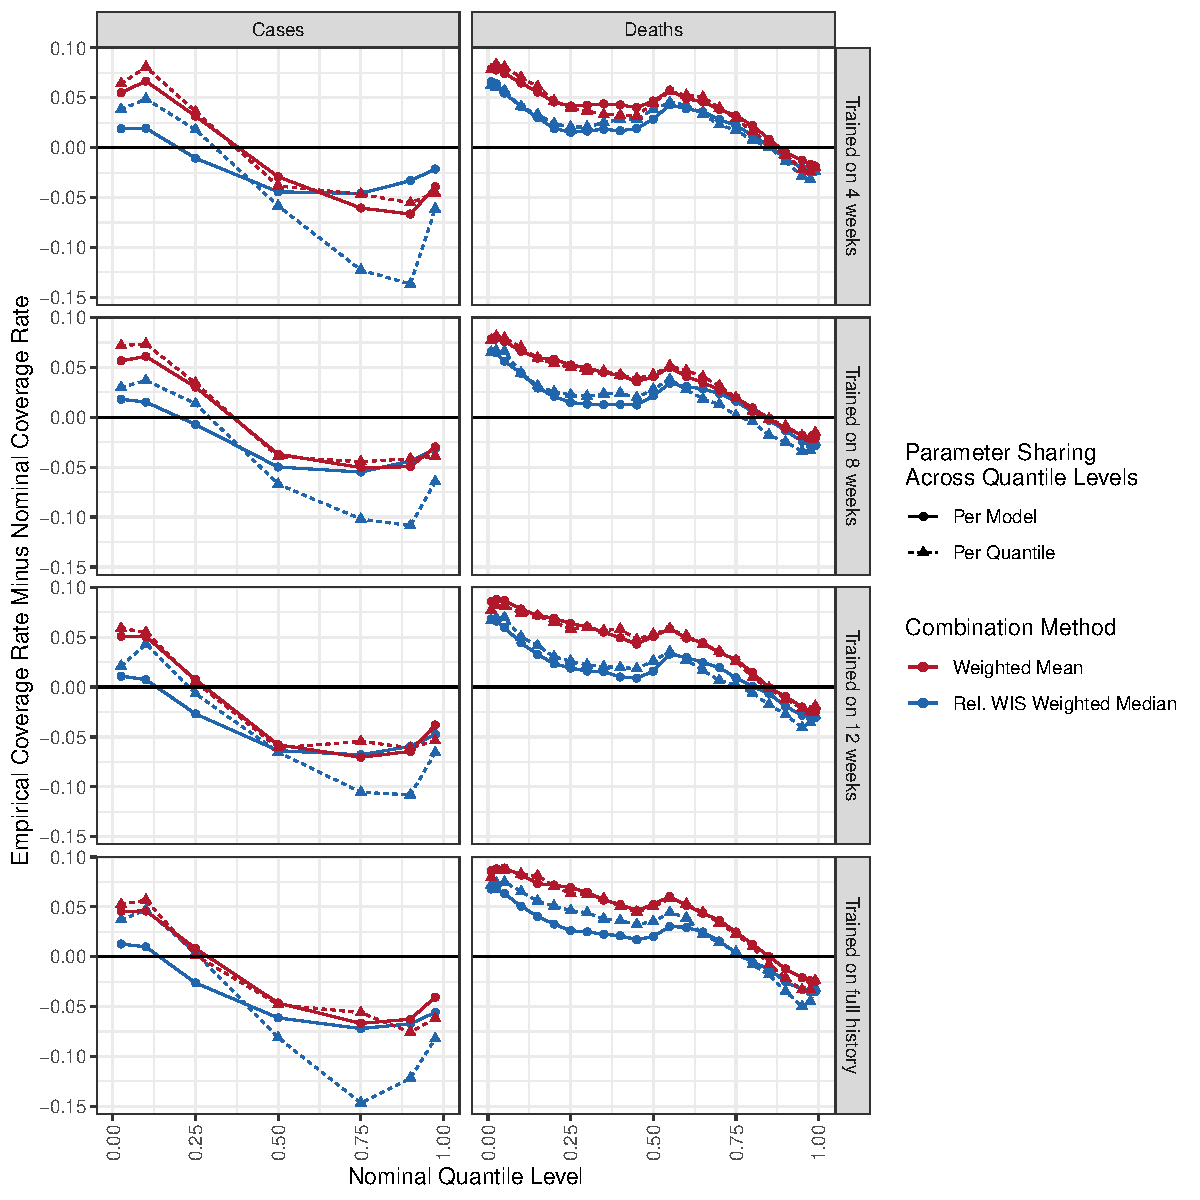
\includegraphics[width=\textwidth]{figures/quantile_coverage_quantile_group.pdf}
  \caption{Quantile coverage rates for the convex weighted mean ensemble and the relative WIS weighted median ensemble, varying whether weights are estimated separately per quantile level (``Per Quantile") or shared across all quantile levels (``Per Model"). All methods combine the top 10 component forecasters in the training set window size specified in facet rows. The vertical axis is the difference between the empirical coverage rate and the nominal coverage rate. A well calibrated method would have a difference of 0 between the empirical and nominal coverage rates, and a method that generates conservative (wide) interval forecasts would have a negative difference for quantile levels less than 0.5 and a positive difference for quantile levels greater than 0.5.}
  \label{fig:coverage_quantile_grouping}
\end{figure}

\newpage

\section{Performance of trained methods near local peaks}

We identified local peaks in state level weekly cases and deaths as weeks that had the maximum incidence within a centered rolling window of 11 weeks (i.e., weeks that had the largest reported weekly counts among the preceding five and following five weeks). By visual inspection, we made manual adjustments to the weeks identified using this rule to remove outliers and weeks that did not correspond to a visually distinct peak. The resulting weeks identified as local peaks are shown in Supplemental Figures~\ref{fig:peak_cases_us_identified} and \ref{fig:peak_deaths_us_identified}. Within our evaluation time frame, there were 159 local peaks for weekly cases and 146 local peaks for weekly deaths across all locations.

\begin{figure}
  \includegraphics[width=\textwidth]{figures/peak_cases_us_identified.pdf}
  \caption{Identified local peaks for weekly cases at the state level. Vertical dashed lines indicate the boundaries of the evaluation phase (the combined model development and prospective evaluation phases). Vertical orange lines indicate the locations of identified local peaks.}
  \label{fig:peak_cases_us_identified}
\end{figure}

\begin{figure}
  \includegraphics[width=\textwidth]{figures/peak_deaths_us_identified.pdf}
  \caption{Identified local peaks for weekly deaths at the state level. Vertical dashed lines indicate the boundaries of the evaluation phase (the combined model development and prospective evaluation phases). Vertical orange lines indicate the locations of identified local peaks.}
  \label{fig:peak_deaths_us_identified}
\end{figure}

Supplemental Figure~\ref{fig:peak_case_death_forecast_errors_by_horizon_central_only} summarizes the central tendency of the errors for predictive medians across all forecasts at the state level in the U.S.\ and for just those forecasts issued in the week before a local peak. The errors are calculated as the value of the predictive median minus the observed count of cases or deaths in the target week, so that errors close to zero are preferred. We show results for three ensemble specifications: the equally weighted median of all component forecasters, the equally weighted median of the top 10 forecasters, and the relative WIS weighted median of the top 10 forecasters. Note that the equally weighted median of all components is untrained, the relative WIS weighted median of the top 10 forecasters is trained, and the equally weighted median of the top 10 forecasters represents an intermediate strategy: it is also trained, but it is not as strongly adaptive to component performance as the weighted median. Both trained ensembles use a training set window size of 12 weeks. We summarize our observations about these errors as follows:
\begin{enumerate}
    \item Across all forecasts of cases, the median error is similar for all three strategies, but the magnitude of the average error from the relative WIS weighted median is slightly larger than the magnitude of the average error from the equally weighted median of all components.
    \item Across all forecasts of deaths, the median error is similar for all three strategies, but the magnitude of the average errors from the relative WIS weighted median is slightly smaller than the magnitude of the average error from the equally weighted median of all components.
    \item For forecasts of cases near peaks, the trained methods were better than the untrained approach in the peak week, but have much larger errors at longer horizons. This indicates that forecasts from the trained methods ``overshot" and missed the turning points by a larger margin than the untrained method.
    \item For forecasts of deaths near peaks, the trained methods have comparable performance to the untrained methods. In contrast to forecasts of cases, training did not exacerbate the tendency to overshoot near local peaks when forecasting deaths.
\end{enumerate}

Supplemental Figure~\ref{fig:peak_case_death_forecast_examples} shows illustrative examples of forecasts made the week before a local peak from the equally weighted median of all components and the relative WIS weighted median of the top 10 components. We can see a systematic tendency for the predictions from the trained method near local peaks to predict a continuation of rising trends for cases, whereas the forecasts of deaths more often capture the coming downturn.

\begin{figure}[H]
  \includegraphics[width=\textwidth]{figures/peak_forecast_errors_cases_deaths_us_no_outliers.pdf}
  \caption{Errors of the predictive median across all forecasts, and for forecasts issued the week before a local peak in weekly cases or deaths. For forecasts issued before a peak, the one week ahead forecasts are for cases in the week of the local peak and forecasts at longer horizons are for cases in weeks after the local peak. The vertical axis is the difference between the predictive median and the observed value. A positive value indicates that the predictive median was larger than the eventually observed value, and a negative value indicates that the predictive median was less than the eventually observed value; a difference of zero is best. Boxes summarize the 25th percentile, median, and 75th percentile of these errors, and crosses show the mean error.}
  \label{fig:peak_case_death_forecast_errors_by_horizon_central_only}
\end{figure}

\begin{figure}
  \includegraphics[width=\textwidth]{figures/peak_forecasts_cases_deaths_us.pdf}
  \caption{Forecast distributions for weekly cases and deaths issued the week before a local peak. Forecasts are shown for all peaks during the evaluation period in the four states with the largest local peaks. Vertical lines indicate the time of the peak, corresponding to the date of a one-week-ahead forecast.}
  \label{fig:peak_case_death_forecast_examples}
\end{figure}

\newpage

\section{Characteristics of component weights in the post hoc weighted mean ensemble}

Supplemental Figure~\ref{fig:post_hoc_weight_characteristics} summarizes characteristics of the component forecaster weights that were obtained from the post hoc weighted mean ensemble. Panel (a) illustrates that in general, the weights were distributed across a larger number of component forecasters in forecasts of deaths than in forecasts of cases. Panel (b) illustrates that the component forecaster weights were only weakly autocorrelated in the post hoc weighted mean ensemble, quantifying the observation that the weights changed substantially from week to week; this can be seen in Figures 4 and 5 in the main text. In contrast, the component forecaster weights were more strongly autocorrelated in the relative WIS weighted mean ensemble. In part, this is due to the use of a 12 week rolling window for estimating component weights; much of the training data for weight estimation is shared in consecutive weeks.

\begin{figure}
  \includegraphics[width=\textwidth]{figures/compare_weight_distributions_and_lag_1_ac.pdf}
  \caption{Characteristics of the component forecaster weights in the post hoc weighted mean ensemble and the relative WIS weighted mean ensemble used in the prospective analysis. Panel (a) shows the number of component forecasters that were required to reach a specified cumulative weight in the post hoc weighted mean ensemble. For example, for cases, in about 95\% of forecast dates at least one component forecaster got weight 0.25 or greater. Panel (b) shows the lag 1 autocorrelation of weight assigned to each component forecaster across weeks. A vertical dashed line shows the mean autocorrelation across all component forecasters.}
  \label{fig:post_hoc_weight_characteristics}
\end{figure}

\newpage

\section{Post hoc evaluation of component weight regularization}

Section 3.4 of the main text describes a post hoc evaluation of regularizing the component forecaster weights in trained ensembles by imposing a limit on the maximum weight that can be assigned to any component. Supplemental Figure~\ref{fig:compare_max_weight_limits_by_date} illustrates that for most forecast dates, imposing this limit on the maximum component weight has negligible effects on the WIS of the ensemble forecasts. However, there are a few forecast dates, particularly concentrated near local peaks for cases, where regularization has a larger impact, with some regularization being helpful for reducing the mean WIS.

\begin{figure}
  \includegraphics[width=\textwidth]{figures/compare_max_weight_limits_by_date.pdf}
  \caption{Mean WIS for state level forecasts of weekly cases and deaths in the United States, where averages for each forecast date are calculated across all locations and forecast horizons. Results are shown for six variations on relative WIS weighted median ensembles that combine the top 10 component forecasters based on a rolling 12 week training set, using different limits for the maximum weight that can be assigned to any component forecaster. A maximum weight limit of 1.0 corresponds to the unregularized approach considered in the prospective analysis in the main text, while a maximum weight limit of 0.1 corresponds to an equal weighting of the ten selected forecasters.}
  \label{fig:compare_max_weight_limits_by_date}
\end{figure}

\newpage

\section{Differences in forecast missingness in the U.S. and Europe}

Supplemental Figures~\ref{fig:case_us_num_locations} through \ref{fig:death_eu_num_locations} show histograms of the number of locations forecasted by the component models contributing to the U.S. COVID-19 Forecast Hub and the European COVID-19 Forecast Hub. Patterns of submission are starkly different for the U.S. and the EU. In the U.S., nearly all models submit forecasts for at least the 50 US States, and many additionally submit forecasts for the District of Columbia and US territories. In the EU, roughly half of forecasters provide forecasts for all or most European countries, while the other half provide forecasts for only a few countries.

Supplemental Figures~\ref{fig:case_us_effective_weights} through \ref{fig:death_eu_effective_weights} show the effective weights used in each location after accounting for forecast missingness by rescaling the weights assigned to available models so that they sum to one. In the U.S., the effective weights closely match the nominal estimated weights in nearly all states, differing only slightly in the territories. In the EU, missingness is more prevalent and it is common for only a few of the selected top 10 component forecasters to provide forecasts for many countries.

\begin{figure}
  \includegraphics[width=\textwidth]{figures/num_locations_per_model_inc_case_state.pdf}
  \caption{Histograms of the number of locations forecasted by each contributing forecaster for weekly cases in the U.S. The top 10 forecasters, indicated with blue shading, were selected for inclusion in the weighted ensembles used for prospective evaluation.}
  \label{fig:case_us_num_locations}
\end{figure}

\begin{figure}
  \includegraphics[width=\textwidth]{figures/num_locations_per_model_inc_death_state.pdf}
  \caption{Histograms of the number of locations forecasted by each contributing forecaster for weekly deaths in the US. The top 10 forecasters, indicated with blue shading, were selected for inclusion in the weighted ensembles used for prospective evaluation.}
  \label{fig:death_us_num_locations}
\end{figure}

\begin{figure}
  \includegraphics[width=\textwidth]{figures/num_locations_per_model_inc_case_euro_countries.pdf}
  \caption{Histograms of the number of locations forecasted by each contributing forecaster for weekly cases in Europe. The top 10 forecasters, indicated with blue shading, were selected for inclusion in the weighted ensembles used for prospective evaluation.}
  \label{fig:case_eu_num_locations}
\end{figure}

\begin{figure}
  \includegraphics[width=\textwidth]{figures/num_locations_per_model_inc_death_euro_countries.pdf}
  \caption{Histograms of the number of locations forecasted by each contributing forecaster for weekly deaths in Europe. The top 10 forecasters, indicated with blue shading, were selected for inclusion in the weighted ensembles used for prospective evaluation.}
  \label{fig:death_eu_num_locations}
\end{figure}

\begin{figure}
  \includegraphics[width=\textwidth]{figures/effective_weights_per_location_inc_case_state.pdf}
  \caption{Component weights for forecasts of weekly cases in the U.S., facetted by forecast date. Only the weights for the first week in each month are shown due to space constraints. The estimated weights that would be used if all models were available for a particular location are shown at left within each facet. The weights actually used for each location are obtained by setting the weight for components that are missing forecasts for that location to 0 and rescaling the others proportionally so that they sum to 1.}
  \label{fig:case_us_effective_weights}
\end{figure}

\begin{figure}
  \includegraphics[width=\textwidth]{figures/effective_weights_per_location_inc_death_state.pdf}
  \caption{Component weights for forecasts of weekly deaths in the U.S., facetted by forecast date. Only the weights for the first week in each month are shown due to space constraints. The estimated weights that would be used if all models were available for a particular location are shown at left within each facet. The weights actually used for each location are obtained by setting the weight for components that are missing forecasts for that location to 0 and rescaling the others proportionally so that they sum to 1.}
  \label{fig:death_us_effective_weights}
\end{figure}

\begin{figure}
  \includegraphics[width=\textwidth]{figures/effective_weights_per_location_inc_case_euro_countries.pdf}
  \caption{Component weights for forecasts of weekly cases in Europe, facetted by forecast date. Only the weights for the first week in each month are shown due to space constraints. The estimated weights that would be used if all models were available for a particular location are shown at left within each facet. The weights actually used for each location are obtained by setting the weight for components that are missing forecasts for that location to 0 and rescaling the others proportionally so that they sum to 1.}
  \label{fig:case_eu_effective_weights}
\end{figure}

\begin{figure}
  \includegraphics[width=\textwidth]{figures/effective_weights_per_location_inc_death_euro_countries.pdf}
  \caption{Component weights for forecasts of weekly deaths in Europe, facetted by forecast date. Only the weights for the first week in each month are shown due to space constraints. The estimated weights that would be used if all models were available for a particular location are shown at left within each facet. The weights actually used for each location are obtained by setting the weight for components that are missing forecasts for that location to 0 and rescaling the others proportionally so that they sum to 1.}
  \label{fig:death_eu_effective_weights}
\end{figure}

\newpage

\section{Adherence to EPIFORGE Guidelines}

\begin{longtable}{c  c  p{9cm}  c}
\toprule
Section & Item & Item Description & Pages \\
\midrule
\endhead
Title/Abstract & 1 & Study described as a forecast or prediction research in at least the title or abstract & 1 \\
\midrule
Introduction & 2 & Purpose of study and forecasting targets defined & 4 \\
\midrule
Methods & 3 & Methods fully documented & 6-13 \\
\midrule
Methods & 4 & Identify whether the forecast was performed prospectively, in real-time, and/or retrospectively & 7 \\
\midrule
Methods & 5 & Origin of input source data explicitly described with reference & 6 \\
\midrule
Methods & 6 & Source data made available, or reasons why this was not possible documented & 13 \\
\midrule
Methods & 7 & Input data processing procedures described in detail & 6-9 \\
\midrule
Methods & 8 & Statement and description of model type, with model assumptions documented with references & 11-13 \\
\midrule
Methods & 9 & Model code made available, or reasons why this was not possible documented & 13 \\
\midrule
Methods & 10 & Description of model validation, with justification of approach. & 6-13 \\
\midrule
Methods & 11 & Description of forecast accuracy evaluation method, with justification & 9-11 \\
\midrule
Methods & 12 & Where possible, compare model results to a benchmark or other comparator model, with justification of comparator choice & 9 \\
\midrule
Methods & 13 & Description of forecast horizon, and justification of its length & 6 \\
\midrule
Results & 14 & Uncertainty of forecasting results presented and explained & 8, 15, 16, 20-22 \\
\midrule
Results & 15 & Results briefly summarized in lay terms, including a lay interpretation of forecast uncertainty & - \\
\midrule
Results & 16 & If results are published as a data object, encourage a time-stamped version number & 13 \\
\midrule
Discussion & 17 & Limitations of forecast described, including limitations specific to data quality and methods & 23, 26, 27 \\
\midrule
Discussion & 18 & If the research is applicable to a specific epidemic, comment on its potential implications and impact for public health action and decision making & 28 \\
\midrule
Discussion & 19 & If the research is applicable to a specific epidemic, comment on how generalizable it may be across populations & 26, 28 \\
\bottomrule
\end{longtable}

\newpage

% Bibliography.
% \section*{References}
\bibliography{bibfile}

\end{document}